\documentclass[]{article}

\usepackage[top=2cm, bottom=2.5cm, left=2.0cm, right=2.0cm]{geometry}
\usepackage{xcolor}
\usepackage{tikz}
\usepackage{pgfplots}
\usepackage{algorithm}
\usepackage{algorithmic}
\usepackage{appendix}
\usepackage{placeins}

\newlength{\xdim}

\definecolor{calculate}{HTML}{D7191C}
\definecolor{copyBack}{HTML}{FDAE61}

%opening
\title{Multiprocessor Systems - Assignment I (MPI)}
\author{Adrian Holfter, Lucie Labadie}

\begin{document}

\maketitle

\section{Implementation}

\subsection{MPI-based Blocked Matrix-Matrix Multiplication}

\paragraph{} Based on the provided one-dimensional row-based implementation, we created an implementation using a two-dimensional block-wise checkerboard data distribution. This means that for two given matrices $A,B$ with $N \times N$ elements each, every worker will compute $m \times n$ values of the result matrix $C$ with $m,n \leq N$.
To compute the result value $C_{m,n}$, the $n$th row of matrix $A$ and the $m$th column of matrix $B$ are needed.
In order to simplify the transfer of the columns of matrix $B$ to the worker nodes, matrix $B$ is transposed in the beginning so it is in column-major order in memory.

\subsection{MPI-based Laplace Approximation}

\paragraph{} First we chose to write the row-wise MPI-implementation of the Laplace Approximation. So we split the matrix on row dimension only given the number of available nodes.
\paragraph{} After splitting the matrix we have to send each part to the workers. Each worker will receive : 
\begin{itemize}
	\item offset : the chunk position in the whole matrix; 
	\item rows : the number of rows the worker have to compute;
	\item matrix : the matrix part the worker should compute with the extra rows and columns needed for the computation (one after and one before). 
\end{itemize}

\paragraph{} Since the original implementation allocates always a memory block of \texttt{MAX\_SIZE} $\times$ \texttt{MAX\_SIZE}, the matrix rows are not adjacent in memory. To circumvent this problem, our implementation dynamically allocates exactly the needed amount of memory, leading to a memory layout in which matrix rows are adjacent. This allows to send multiple rows at once and helps to avoid excessive amounts of \texttt{MPI\_Send()} calls.

\paragraph{} The master will then do its part of the computation and wait to receive the results of the workers. 

\paragraph{} The workers will receive their data and start the computation, after computation they will send back the results to the master : 
\begin{itemize}
	\item offset;
	\item result matrix.
\end{itemize}
We do not need to send the number of rows again since it is already known by the master. 

\paragraph{} The work executed by each worker and the master starts by exchanging the extra rows on top and bottom. During the first turn this operation is not really necessary but it will serve for the next since it is needed for the further computations. The first pass of computation is executed respecting the turn we are in (ODD or EVEN). The stopping condition is checked by taking the maximum of each row and keeping only the biggest sum. If this sum is converging (difference between two runs of the same type approaches $0$), the computation is stopped. To do so, each worker is computing its own maximum value and sends it to the master which will check whether to stop or not and send the result back the workers. Then the turn type is switched (ODD or EVEN) and another iteration is started.

\section{Measurements}

The measurements were taken on the \emph{kraken.tek.bth.se} Server. The executables were compiled with the \texttt{-O2} option, to enable compiler optimizations. Every measurement was taken 10 times and the smallest value was used to account for background load and operating system caches.

\subsection{MPI-based Blocked Matrix-Matrix Multiplication}

 Table \ref{tab:matrix-mult-runtime} shows the runtimes of the different versions of the blocked matrix-matrix multiplication.

\begin{figure}[h]
	\centering
	\begin{tabular}{|l|r|r|}
		\hline
		\textbf{Version} & \textbf{shortest runtime [s]} & \textbf{speedup} \\
		\hline
		Sequential single-threaded	& 30.40	& 1.0 \\ 
		\hline 
		MPI 1 thread				& 2.54	& 11.97 \\ 
		\hline 
		MPI 2 threads				& 0.95	& 32.00 \\ 
		\hline 
		MPI 4 threads				& 0.57	& 53.33 \\ 
		\hline 
		MPI 8 threads				& 0.47	& 64.68 \\ 
		\hline 
	\end{tabular} 
	\caption{Runtime comparison for matrix multiplication}
	\label{tab:matrix-mult-runtime}
\end{figure}

There is a substantial speedup noticeable for the MPI version in comparison to the original sequential values, even when running single-threaded. The explanation for this is most probably that the matrix $B$ is now stored in column-major order in memory, which means that the memory layout now more closely matches the access pattern, allowing for a far better cache-hit ratio.

Figure \ref{fig:maxtrix-mult-chart} shows the runtime breakdown for the MPI version per number of workers. It becomes clear that the percentage of time spent copying back the result matrix increases rapidly, which is because every worker sends back the \emph{whole} \texttt{C} matrix, even though only a small part of it actually contains work results.

\begin{figure}[h]
	\centering
	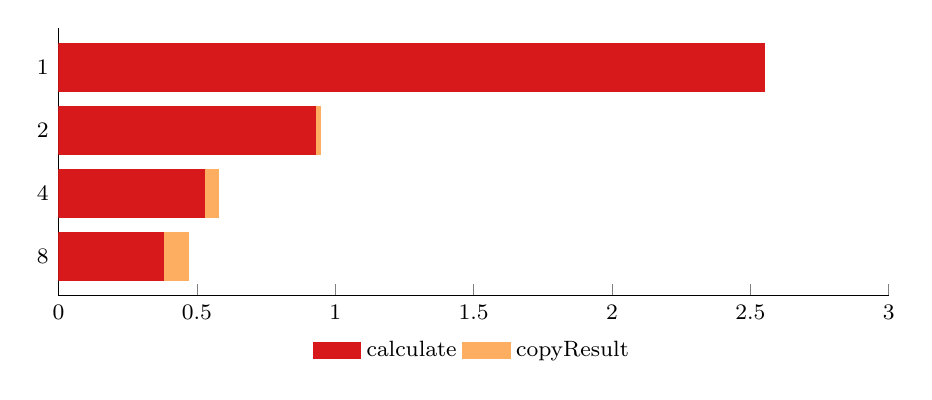
\begin{tikzpicture}
	\begin{axis}[
	xbar stacked,
	legend style={
		legend columns=4,
		at={(xticklabel cs:0.5)},
		anchor=north,
		draw=none
	},
	ytick=data,
	axis y line*=none,
	axis x line*=bottom,
	tick label style={font=\footnotesize},
	legend style={font=\footnotesize},
	label style={font=\footnotesize},
	xtick={0, 0.5, 1.0, 1.5, 2.0, 2.5, 3.0},
	width=1.0\textwidth,
	bar width=6mm,
	xlabel={Time in s},
	yticklabels={1, 2, 4, 8},
	xmin=0,
	xmax=3.0,
	area legend,
	y=8mm,
	enlarge y limits={abs=0.625},
	]
	\addplot[calculate,fill=calculate] coordinates
	{(2.55,3) (0.927,2) (0.527,1) (0.380,0)};
	\addplot[copyBack,fill=copyBack] coordinates
	{(0.0,3) (0.02,2) (0.05,1) (0.09,0)};
	\legend{calculate, copyResult}
	\end{axis}  
	\end{tikzpicture}
	\caption{Runtime breakdown for matrix multiplication per number of workers}
	\label{fig:maxtrix-mult-chart}
\end{figure}

\subsection{MPI-based LaPlace Approximation}

 Table \ref{tab:laplace-sor-runtime} shows the runtimes of the different versions of the row-based LaPlace approximation using successive over-relaxation. Figure \ref{fig:laplace-sor-chart} also visualizes this.

\begin{figure}[h]
	\centering
	\begin{tabular}{|l|r|r|}
		\hline
		\textbf{Version} & \textbf{shortest runtime [s]} & \textbf{speedup} \\
		\hline
		Sequential single-threaded	& 41.03 & 1.00 \\ 
		\hline 
		MPI 1 thread				& 41.42 & 0.99 \\ 
		\hline 
		MPI 2 threads				& 23.85 & 1.72 \\ 
		\hline 
		MPI 4 threads 				& 16.45 & 2.49 \\ 
		\hline 
		MPI 8 threads				& 13.56 & 3.05 \\ 
		\hline 
	\end{tabular} 
	\caption{Runtime comparison for LaPlace approximation}
	\label{tab:laplace-sor-runtime}
\end{figure}

\begin{figure}[h]
	\centering
	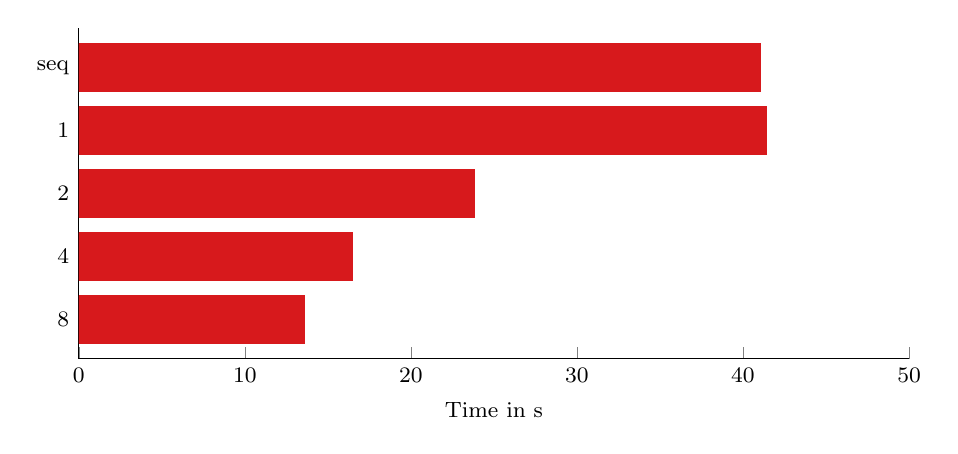
\begin{tikzpicture}
	\begin{axis}[
	xbar stacked,
	legend style={
		legend columns=4,
		at={(xticklabel cs:0.5)},
		anchor=north,
		draw=none
	},
	ytick=data,
	axis y line*=none,
	axis x line*=bottom,
	tick label style={font=\footnotesize},
	legend style={font=\footnotesize},
	label style={font=\footnotesize},
	xtick={0, 10.0, 20.0, 30.0, 40.0, 50.0},
	width=1.0\textwidth,
	bar width=6mm,
	xlabel={Time in s},
	yticklabels={seq, 1, 2, 4, 8},
	xmin=0,
	xmax=50.0,
	area legend,
	y=8mm,
	enlarge y limits={abs=0.625},
	]
	\addplot[calculate,fill=calculate] coordinates
	{(41.03,4) (41.42,3) (23.85,2) (16.45,1) (13.56, 0)};
	\end{axis}  
	\end{tikzpicture}
	\caption{Runtime comparison chart for LaPlace approximation}
	\label{fig:laplace-sor-chart}
\end{figure}

\FloatBarrier

\begin{appendix}
	\section*{Appendix A: Matrix multiplication algorithm}
	something
	\section*{Appendix B: Laplace Approximation global algorithm}
	\begin{algorithm}
		\caption{Laplace Approximation row-wise parallel implementation : global algorithm}
		\label{laplace}
		\begin{algorithmic}
			\STATE MPI initialize
			\STATE matrix initialize
			\STATE split the matrix
			\IF{master} 
			\FOR{p from 1 to number of cores}
			\STATE MPI Send(offset to worker p)
			\STATE MPI Send(number of rows to worker p)
			\STATE MPI Send(matrix to worker p)
			\ENDFOR
			\STATE Call work(number of rows, offset)
			\FOR{p from 1 to number of cores}
			\STATE MPI Recv(offset from worker p)
			\STATE MPI Recv(matrix from worker p)
			\ENDFOR
			\ELSE 
			\STATE MPI Recv(offset from master)
			\STATE MPI Recv(number of rows from master)
			\STATE MPI Recv(matrix from master)
			\STATE Call work(number of rows, offset)
			\STATE MPI Send(offset to master)
			\STATE MPI Send(matrix to master)
			\ENDIF
			\STATE MPI finilize
		\end{algorithmic}
	\end{algorithm}
	\section*{Appendix C: Laplace Approximation work algorithm}
	\begin{algorithm}
		\caption{Laplace Approximation row-wise parallel implementation : work function}
		\label{laplace_work}
		\begin{algorithmic}
			\STATE turn = EVEN
			\WHILE {not finished}
			\STATE iteration++
			\IF{not the first row}
			\STATE MPI Recv(top row from above worker)
			\STATE MPI Send(top row to above worker)
			\ENDIF
			\IF{not the last row}
			\STATE MPI Send(bottom row to below worker)
			\STATE MPI Recv(bottom row from below worker)
			\ENDIF
			\STATE Computations Laplace Approximation
			\STATE Max row sum calculation
			\IF{not the master}
			\STATE MPI Send(max row sum to master)
			\ELSE 
			\STATE Check stopping conditions
			\ENDIF
			\STATE MPI Broadcast(finished status to every worker)
			\STATE turn changing 
			\ENDWHILE
			\RETURN iteration
		\end{algorithmic}
	\end{algorithm}
\end{appendix}

\end{document}